\begin{document}

A useful information of the study of the temperature in Sweden is to look for the warmest and the coldest day at different locations in Sweden. The dates of the warmest and coldest day fluctuate every year, while it is assumed that its overall distribution is Gaussian-like. In this section, we use provided data from all locations to explore the distribution of the warmest and the coldest day of each year in Sweden. 

\subsection{Method}
In order to get the highest and the lowest temperature, the temperature data from the same year is scanned through. At the first day of a year, the minimum and maximum temperature is assigned to the temperature of the first day. If the temperature of the second day is either larger or smaller than the maximum or the minimum temperature, the maximum or the minimum temperature is updated, respectively. By comparing the temperature of consecutive days with the constantly updated minimum and maximum temperature, the warmest and coldest day of a year can be determined. The complexity of such algorithm is linear with respect to the data size. As the date is stored in the normal calendar format, year-month-day, it is necessary to convert it into the day of the year so as to quantify the date. This is done by creating the \texttt{getDayOfYear} function in \texttt{tempTrender.cpp}, which takes into account of leap years.  

The distribution of the warmest and coldest day of a year are plotted in the same histogram and are fitted to a Gaussian. It can be seen in the result section below that the distribution of the coldest day of a year ranges from the end of November to the start of March, so that the histogram for the coldest day is not continuous, but scattered at the two ends of the histogram. In order to fit a Gaussian to it, which joins the two ends, two histograms for the coldest day are created and each one is filled with the complete data of the coldest day, as shown in Fig. \ref{hotColdUppsalaFit}.
\begin{figure}[H]
\centering
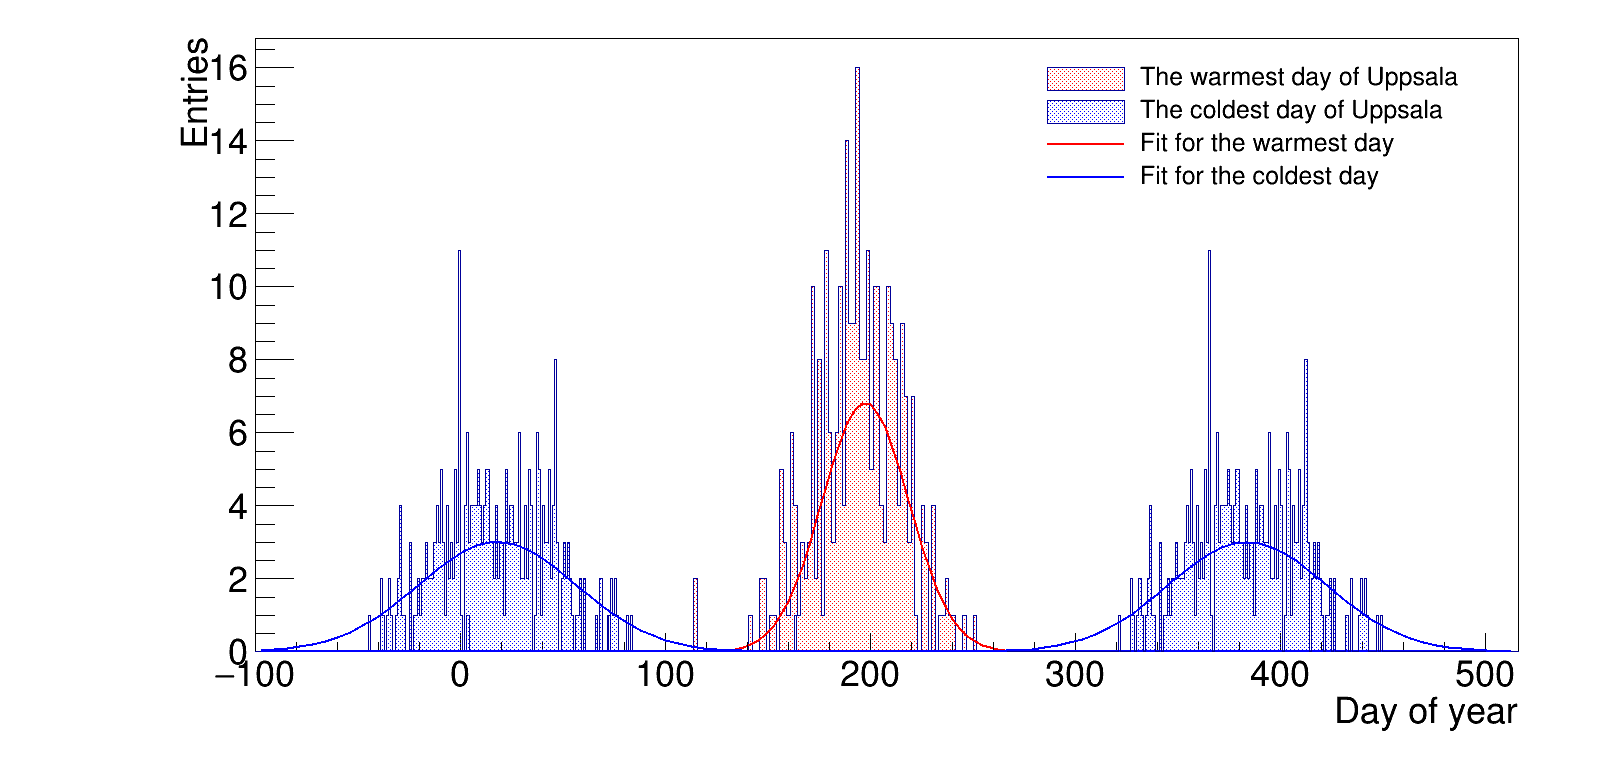
\includegraphics[scale=.25,trim=5cm 0cm 0 0]{hotCold_Uppsala_entire.png}
\caption{A demonstration of the method we used to fit the distribution of the coldest day of a year. }
\label{hotColdUppsalaFit}
\end{figure}

\subsection{Results}
The distribution of the warmest and the coldest day for Uppsala, Lund and Lulea are shown in Fig. \ref{hotColdUppsala}, \ref{hotColdLund} and \ref{hotColdLulea}, respectively. The number of years in Uppsala data is around six times more than that in other data files. This gives a lot more entries to the plot of Uppsala, so that its Gaussian fit has the best $\chi^2$ value (around 0.9). Since other data files generally only have 50 to 60 entries in total, the bin number is reduced from 366 for Uppsala to 50 so as to have more entries in each bin. Due to insufficient number of data, the $\chi^2$ for locations other than Uppsala generally varies significantly with the choice of the number of bins. We pick Lund and Lulea as two sample places to show the plot of the warmest- and coldest-day distribution, with Lund corresponding to one of the places at the lowest latitude and Lulea corresponding to the place at the highest latitude from the data provided. It can be seen that the coldest day in Lulea ($22^{th}$ Jan) is about the same as Lund ($23^{th}$ Jan.), while the hottest day in Lulea is three days earlier than that in Lund ($15^{th}$ July). 

The results of the mean of the warmest and the coldest with corresponding uncertainty is summarized in Table \ref{hotColdResult}. The order of the place in the table is chosen to start from low latitude to high latitude. However, there is no clear relation between the mean value of the warmest and coldest day to the latitude.

\begin{figure}[H]
\centering
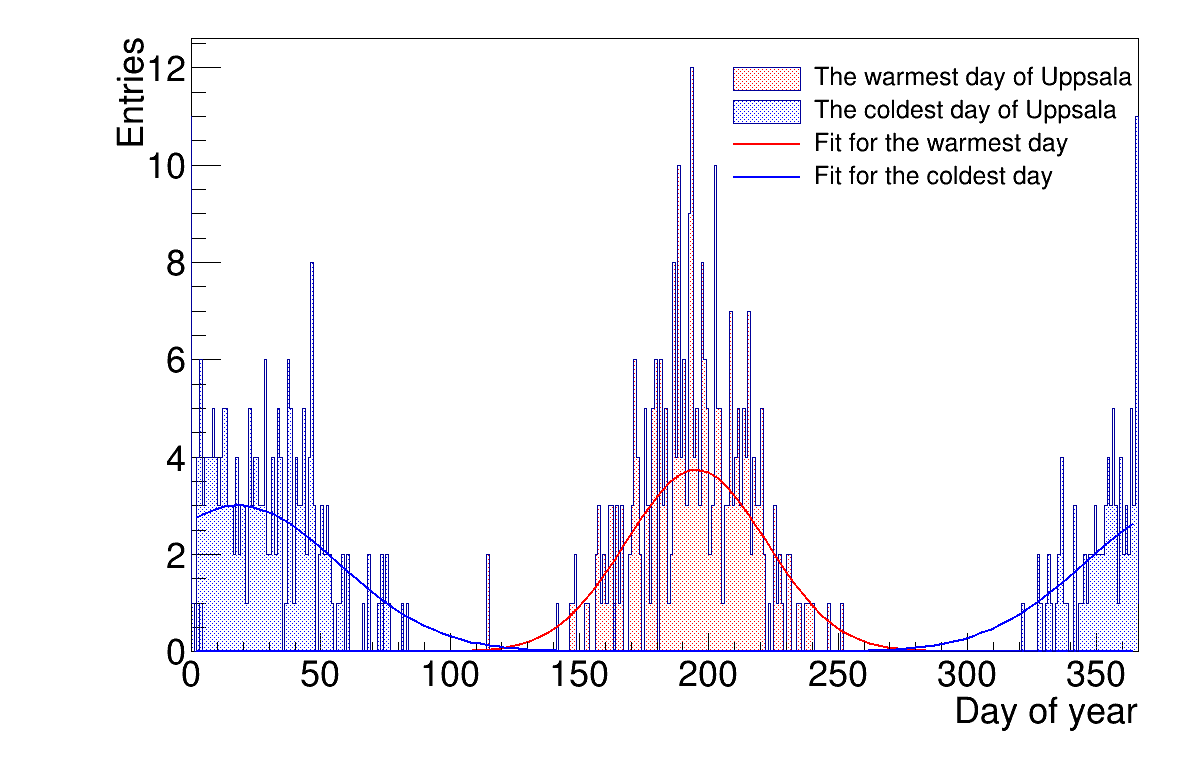
\includegraphics[width=0.7\textwidth]{hotCold_Uppsala.png}
\caption{The distribution of the warmest and the coldest day for each year in Uppsala from 1722 to 2013. A Gaussian function is fit to each of the distribution with $\chi^2/\text{dof}$ determined to be 0.90. Note that the temperature for some years was not recorded or partially recorded for Uppsala. Only the data that are strictly from Uppsala are read by the \texttt{readData} function. }
\label{hotColdUppsala}
\end{figure}

\begin{figure}[H]
\centering
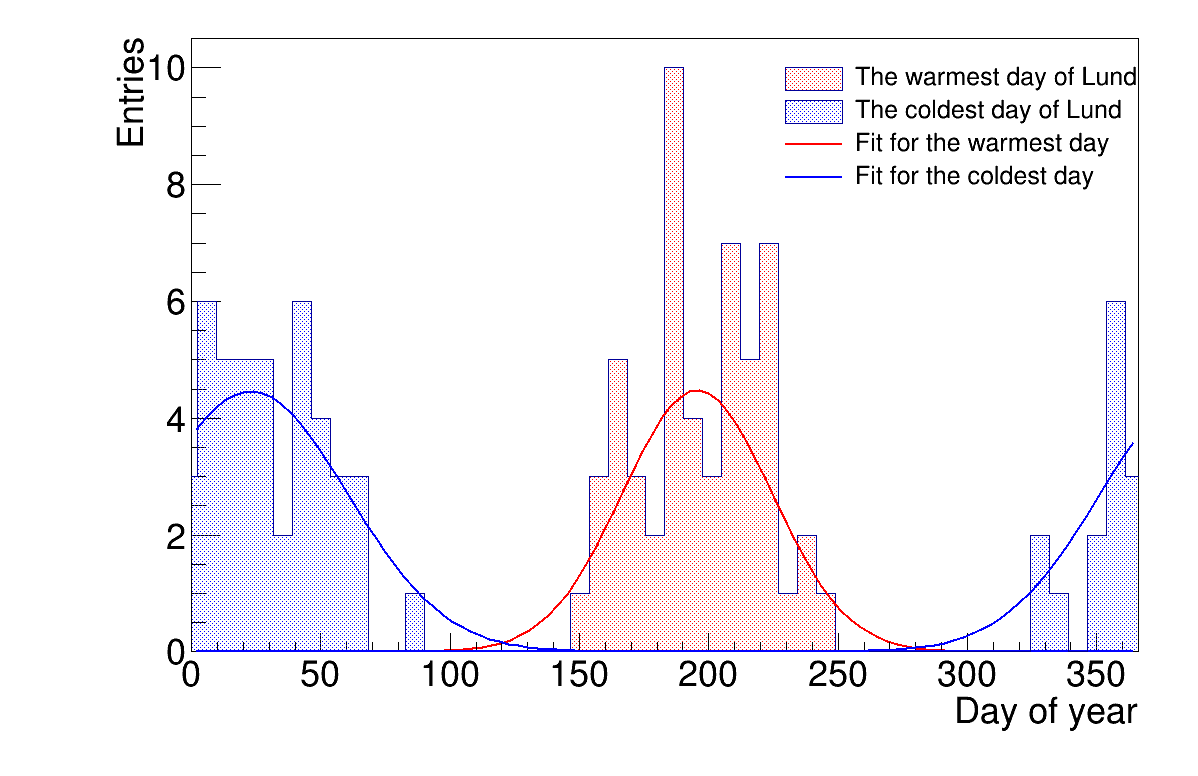
\includegraphics[width=0.7\textwidth]{hotCold_Lund.png}
\caption{The distribution of the warmest and the coldest day for each year in Lund from 1961 to 2015. A Gaussian function is fit to each of the distribution with $\chi^2/\text{dof}$ determined to be 1.18.}
\label{hotColdLund}
\end{figure}

\begin{figure}[H]
\centering
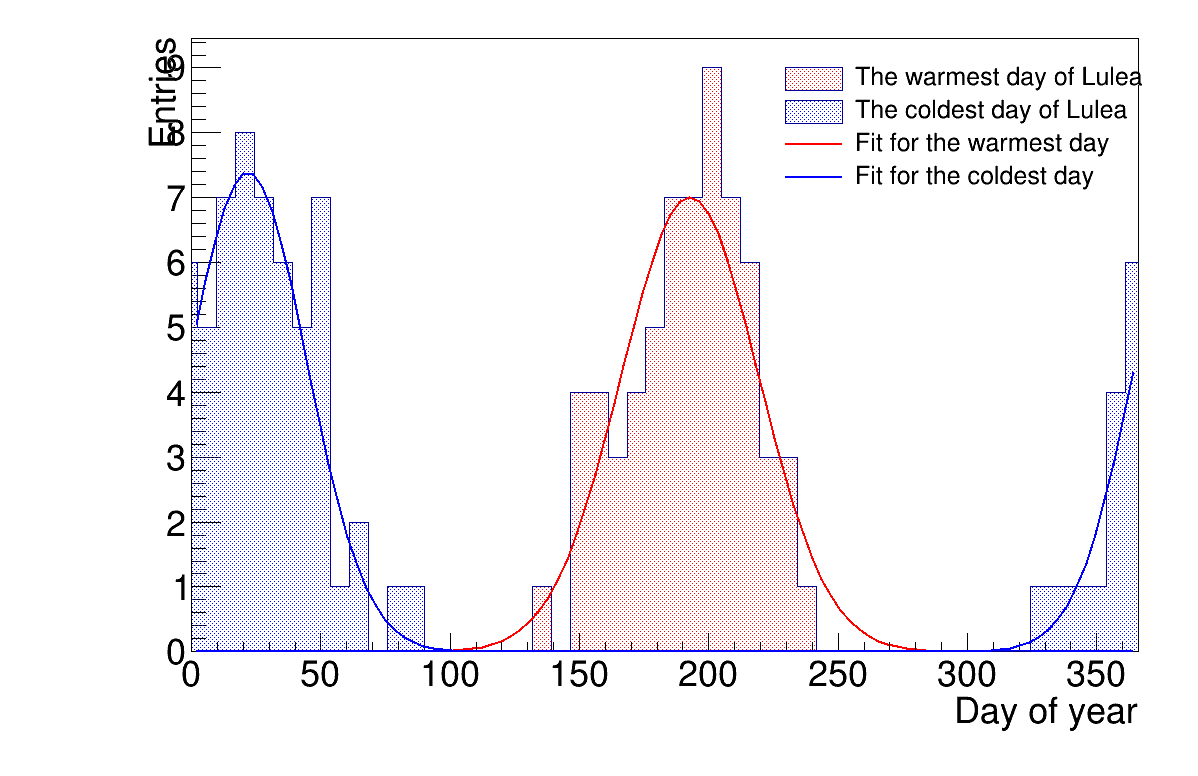
\includegraphics[width=0.7\textwidth]{hotCold_Lulea.png}
\caption{The distribution of the warmest and the coldest day for each year in Lulea from 1951 to 2015. A Gaussian function is fit to each of the distribution with $\chi^2/\text{dof}$ determined to be 0.37.}
\label{hotColdLulea}
\end{figure}

\begin{table}[H]
\centering
\begin{tabular}{p{1.7cm} p{2.0cm} p{2.2cm} p{2.0cm} p{2.3cm}}
\hline
  & Mean of the warmest day & Uncertainty of mean of the warmest day & Mean of the coldest day & Uncertainty of the mean of the coldest day \\ \hline \hline
Falsterbo & 198.9                   & 3.8                                    & 28.6                    & 5.4                                        \\ \hline
Lund      & 195.5                   & 5.7                                    & 22.9                    & 4.9                                        \\ \hline
Visby     & 197.8                   & 4.0                                    & 44.3                    & 9.0                                        \\ \hline
Boras     & 188.6                   & 4.9                                    & 29.0                    & 13.4                                       \\ \hline
Soderarm  & 209.1                   & 2.9                                    & 34.6                    & 3.7                                        \\ \hline
Karlstad  & 199.9                   & 4.8                                    & 25.5                    & 11.4                                       \\ \hline
Uppsala   & 195.1                   & 2.4                                    & 17.9                    & 3.7                                        \\ \hline
Falun     & 196.8                   & 4.8                                    & 19.1                    & 7.0                                        \\ \hline
Umea      & 200.1                   & 6.0                                    & 29.6                    & 4.7                                        \\ \hline
Lulea     & 192.7                   & 4.4                                    & 21.8                    & 3.2                                        \\ \hline
\end{tabular}
\caption{Calculation of the mean of the warmest day and the coldest day from the Gaussian fit. The uncertainty for each mean value is evaluated. The order of the place is chosen to start from low latitude to high latitude. }
\label{hotColdResult}
\end{table}

\end{document}
